\documentclass[tikz,border=10pt]{standalone}
\usetikzlibrary{angles}

\begin{document}
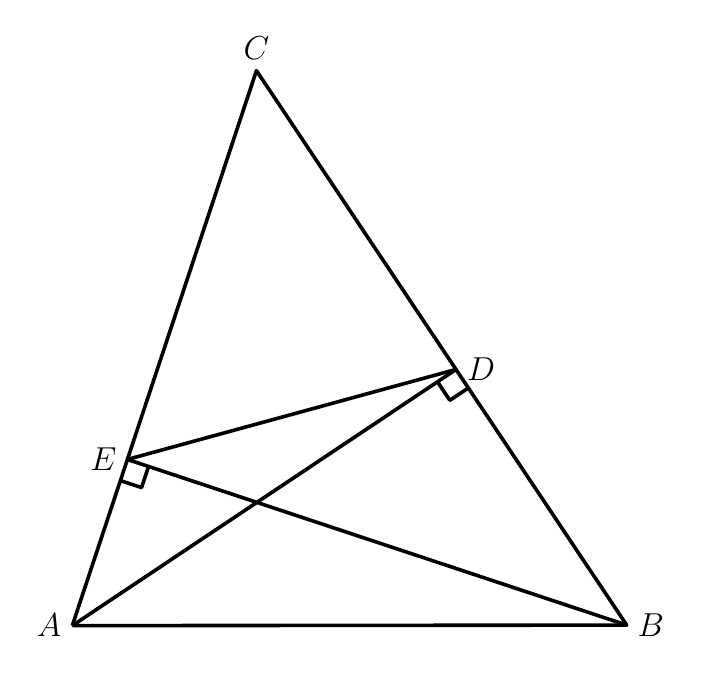
\begin{tikzpicture}[line width=1.3pt, line join=round]
\coordinate (A) at (-3.538,-3.673);
\coordinate (B) at (3.503,-3.666);
\coordinate (C) at (-1.199,3.376);
\coordinate (D) at (1.335,-0.419);
\coordinate (E) at (-2.838,-1.562);

  

  
  \draw (A) -- (E) -- (C) -- (D) -- (B) -- (A);

  
  \draw (A) -- (D);
  \draw (B) -- (E);
  \draw (D) -- (E);

  
  \draw pic[draw, angle radius=0.283cm] {right angle=A--D--B};
  \draw pic[draw, angle radius=0.283cm] {right angle=A--E--B};

  
  \node[above, font=\fontsize{11.5}{13.8}\selectfont] at (C) {$C$};
  \node[left,  font=\fontsize{11.5}{13.8}\selectfont] at (A) {$A$};
  \node[right, font=\fontsize{11.5}{13.8}\selectfont] at (B) {$B$};
  \node[right, font=\fontsize{11.5}{13.8}\selectfont] at (D) {$D$};
  \node[left,  font=\fontsize{11.5}{13.8}\selectfont] at (E) {$E$};
\end{tikzpicture}
\end{document}